
\section{Optimization Algorithm Performance Analysis} \label{app:knot-selection}

This appendix provides comprehensive visualization of optimization algorithm performance across all six data-generating processes (DGPs) and basis orders. The figures show both knot selection behavior and loss convergence patterns for four optimization algorithms: FISTA, ProximalAdaGrad, ProximalNewton, and ProximalNewtonLBFGS, compared against the \texttt{CVXPY} reference solution.

\subsection{Notation and setup}
We denote by $n$ the number of samples, $G$ the number of midpoint intervals used for normalization on $[0,1]$, $k \in \{0,1,2\}$ the basis order, $K$ the total number of basis coefficients (intercept, $k$ polynomial terms, and $M$ truncated\,-\,power terms), $s$ the active set size used in coordinate descent, and $L_k$ the number of objective evaluations performed by backtracking at iteration $k$. Throughout, matrix\,-\,vector multiplies with dense $a\times b$ arrays are costed as $2ab$ FLOPs.

\subsection{Per-iteration FLOP derivations}
We summarize implementation\,-\,aware FLOP counts for each algorithm; see the project note \path{experiments/compare_knot_selection/algorithm_flop_per_iter.md} in the experiment git repo for additional commentary and logging details.

\paragraph{FISTA} A forward pass on data and midpoints and a backward pass via autograd each cost $\Theta\big((n+G)K\big)$, with an additional $\Theta(GK)$ for the exact normalization update. Dominant term: $\Theta\big((n+G)K\big)$.

\paragraph{Proximal AdaGrad} Computing the gradient uses $\Theta\big(nK + GK\big)$; forming the diagonal Hessian via variance on midpoints contributes another $\Theta(GK)$ (tighter bound) to $\Theta(3GK)$ (conservative). Including the normalization step yields a dominant $\Theta\big((n+G)K\big)$.

\paragraph{Proximal Newton (full)} Each iteration forms the gradient in $\Theta\big((n+G)K\big)$, the Hessian as a weighted covariance on midpoints in $\Theta\big(GK^2\big)$, solves the proximal subproblem via coordinate descent in $\Theta\big(sK^2\big)$, and performs $L_k$ objective evaluations contributing $\Theta\big(L_k (n+G)K\big)$; normalization adds $\Theta(GK)$. Dominant term: $\Theta\big(GK^2 + sK^2\big) + \Theta\big((1+L_k)(n+G)K\big)$.

\paragraph{Proximal Newton L\,-\,BFGS} Replacing the full Hessian with an L\,-\,BFGS update avoids the $GK^2$ term; per iteration is dominated by the gradient and line search plus normalization: $\Theta\big((1+L_k)(n+G)K\big)$.

\subsection{From iterations to cumulative FLOPs}
Given per\,-\,iteration FLOP estimates $F(k)$, cumulative FLOPs up to iteration $t$ are $C(t) = \sum_{k=1}^t F(k)$. Our visualization utilities infer $L_k$ from logged step sizes $\alpha_k$ (with backtracking factor $\beta=0.5$) and use consistent baselines at iteration/FLOP zero. See the note for practical defaults and alignment details.

\begin{figure}[H]
    \centering
    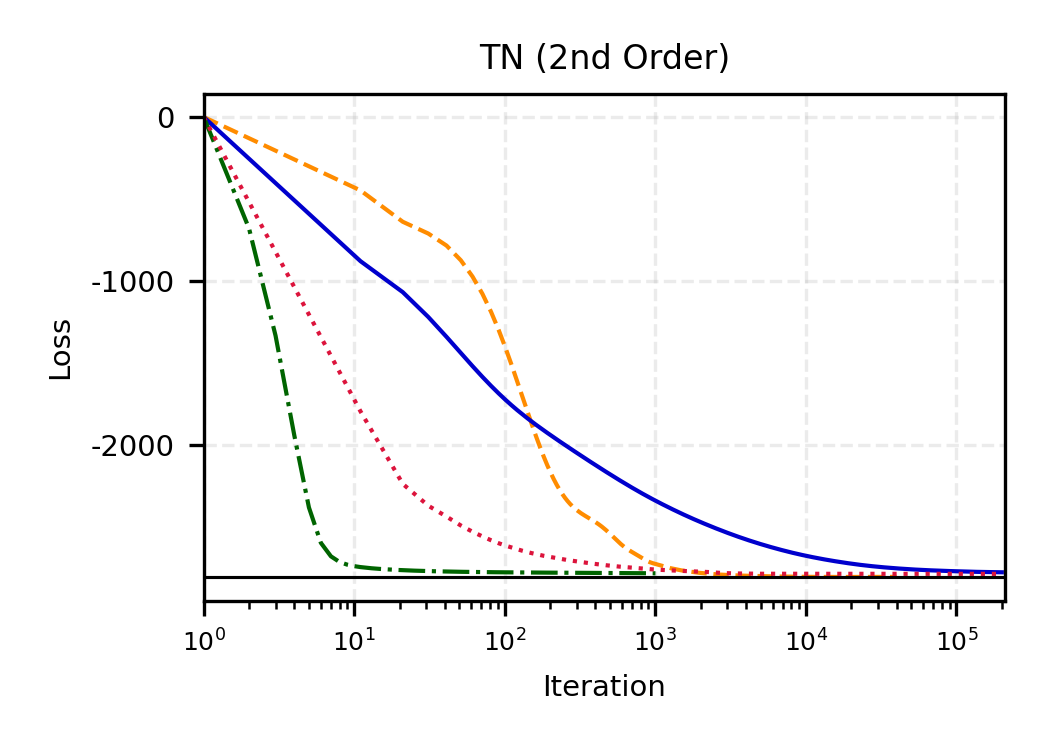
\includegraphics[width=.49\textwidth]{resources/optimization_algorithms/per_iter/TruncatedNormal_order_2_loss_per_iter.png}
    \hfill
    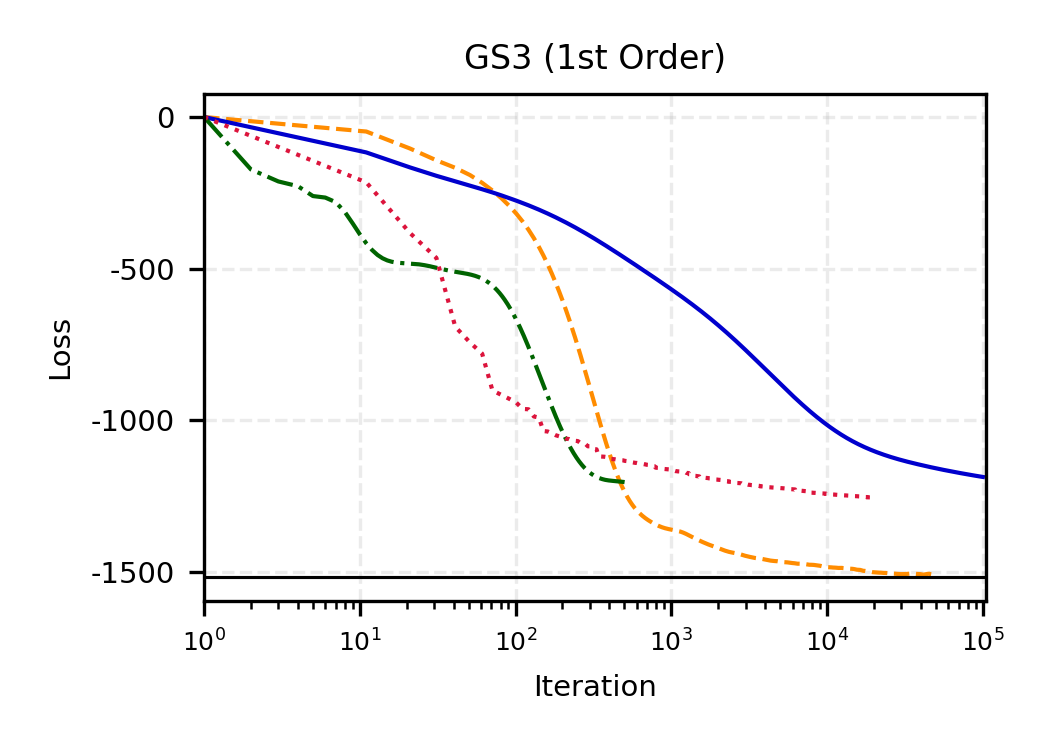
\includegraphics[width=.49\textwidth]{resources/optimization_algorithms/per_iter/TruncatedGMMSymmetricThree_order_1_loss_per_iter.png}
    
    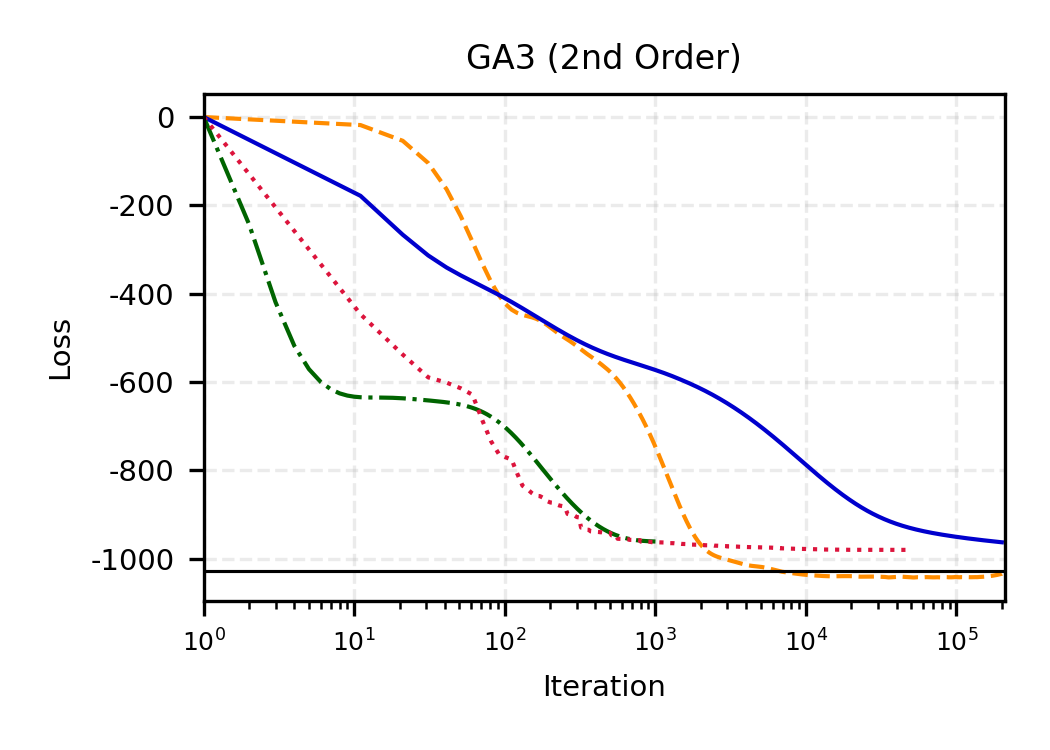
\includegraphics[width=.49\textwidth]{resources/optimization_algorithms/per_iter/TruncatedGMMAsymmetricThree_order_2_loss_per_iter.png}
    \hfill
    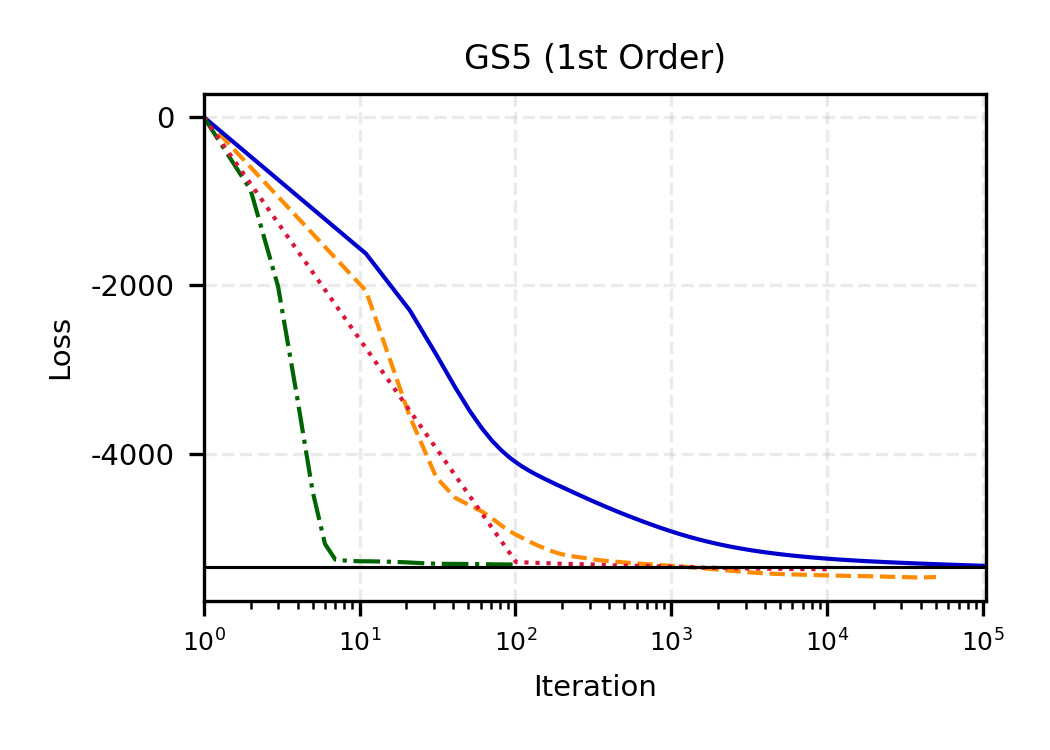
\includegraphics[width=.49\textwidth]{resources/optimization_algorithms/per_iter/TruncatedGMMFiveSpikes_order_1_loss_per_iter.png}
    
    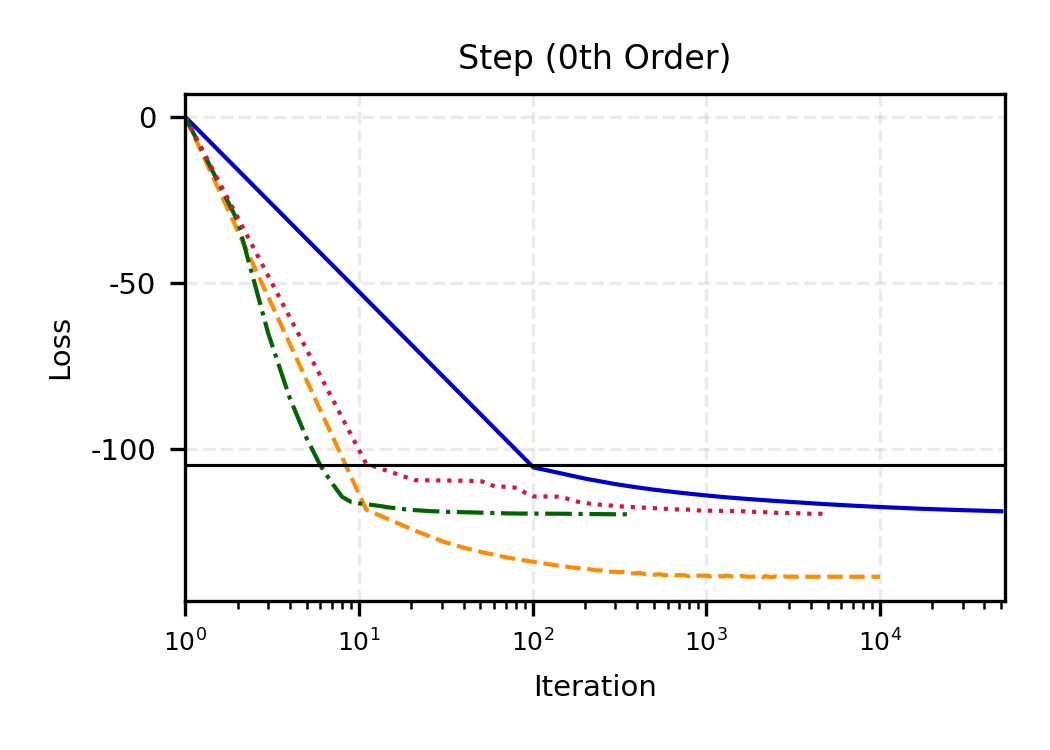
\includegraphics[width=.49\textwidth]{resources/optimization_algorithms/per_iter/StepFunction_order_0_loss_per_iter.png}
    \hfill
    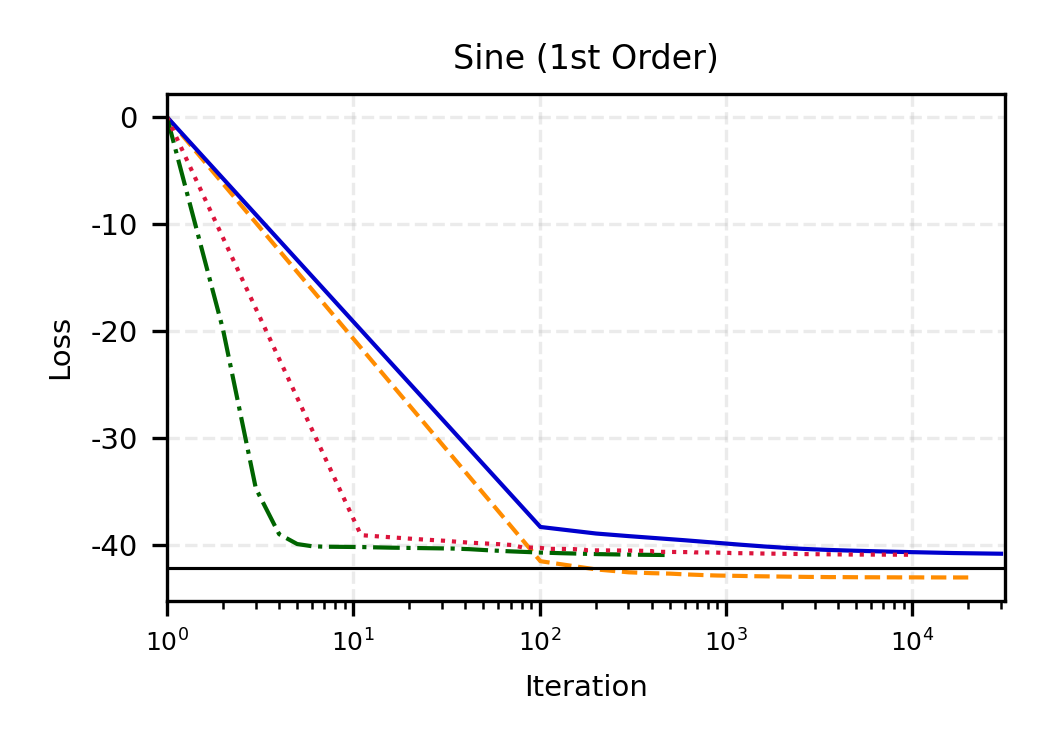
\includegraphics[width=.49\textwidth]{resources/optimization_algorithms/per_iter/Sinusoidal_order_1_loss_per_iter.png}
    
    \caption{Per-iteration loss convergence for optimization algorithms across six DGPs. Panels (row-wise, left to right): (a) TN, (b) GS3, (c) GA3, (d) GS5, (e) Step, (f) Sine.}
    \label{fig:opt-per-iter-loss}
    \end{figure}
    
    \begin{figure}[H]
    \centering
    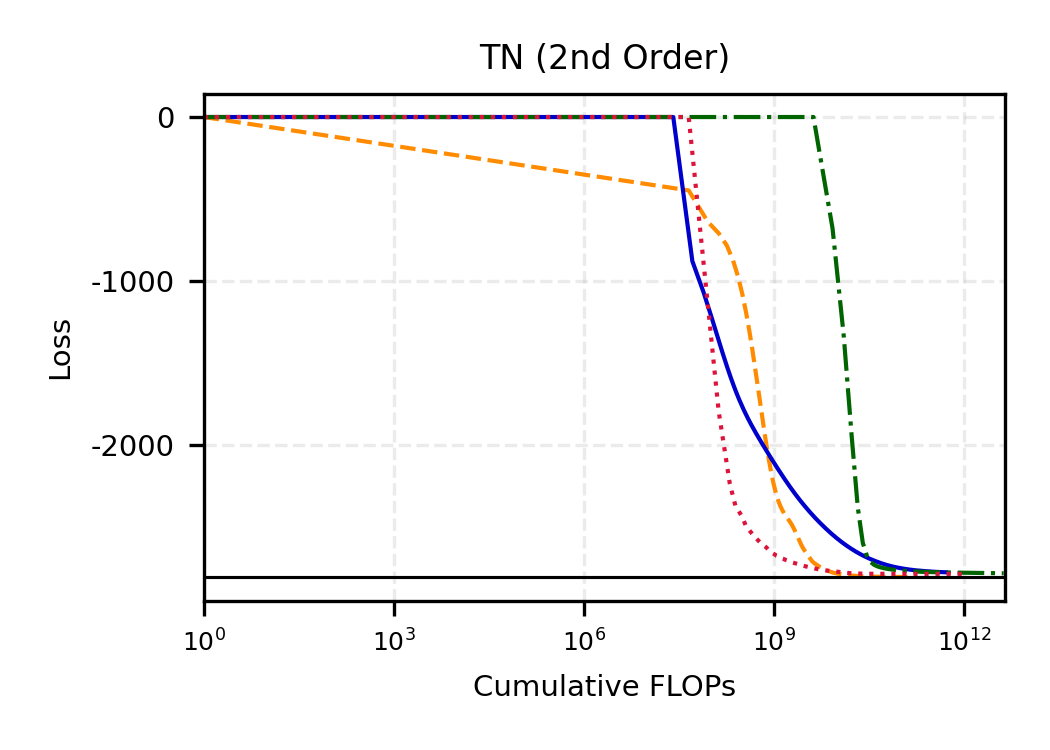
\includegraphics[width=.49\textwidth]{resources/optimization_algorithms/per_flop/TruncatedNormal_order_2_loss_per_flop.png}
    \hfill
    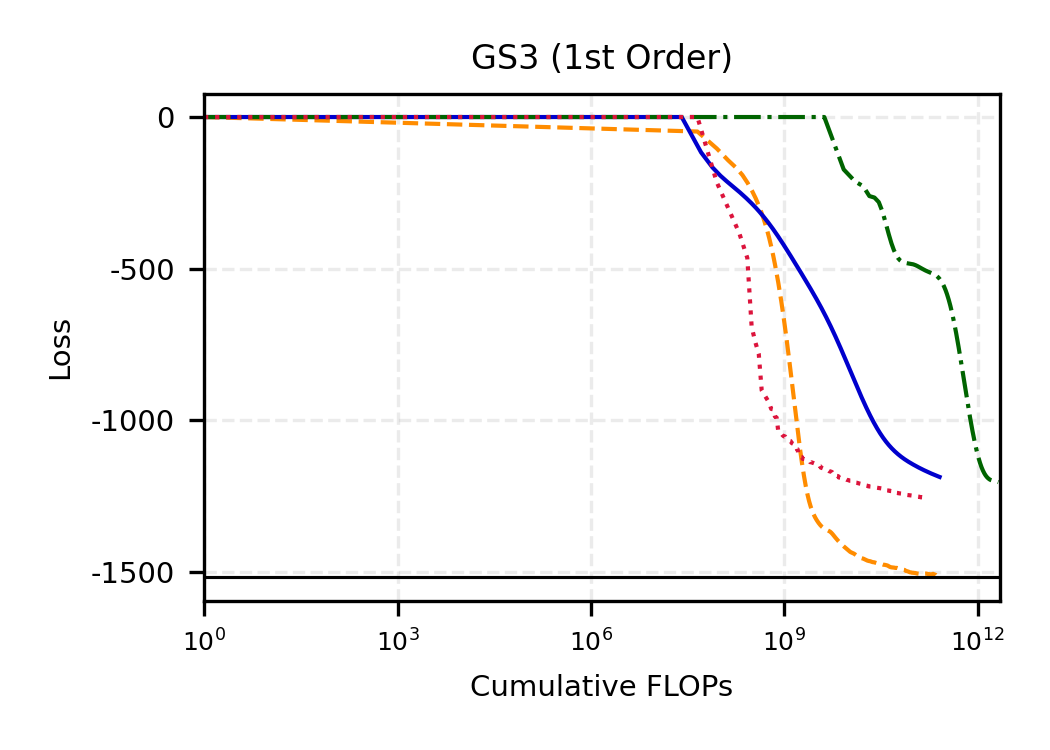
\includegraphics[width=.49\textwidth]{resources/optimization_algorithms/per_flop/TruncatedGMMSymmetricThree_order_1_loss_per_flop.png}
    
    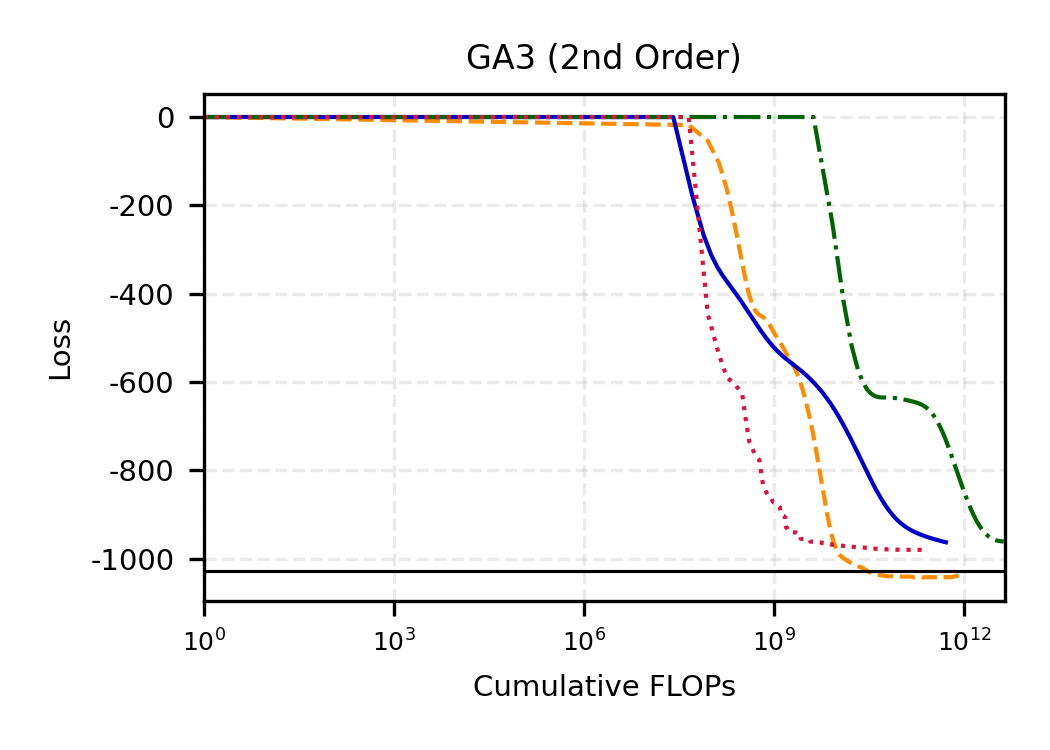
\includegraphics[width=.49\textwidth]{resources/optimization_algorithms/per_flop/TruncatedGMMAsymmetricThree_order_2_loss_per_flop.png}
    \hfill
    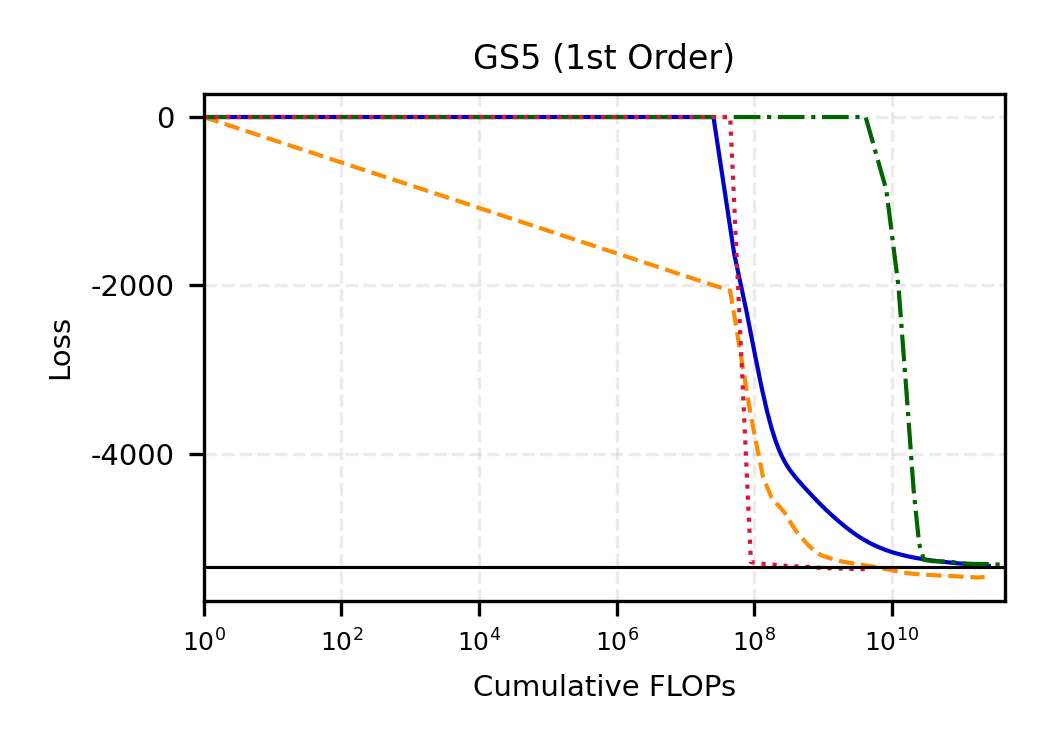
\includegraphics[width=.49\textwidth]{resources/optimization_algorithms/per_flop/TruncatedGMMFiveSpikes_order_1_loss_per_flop.png}
    
    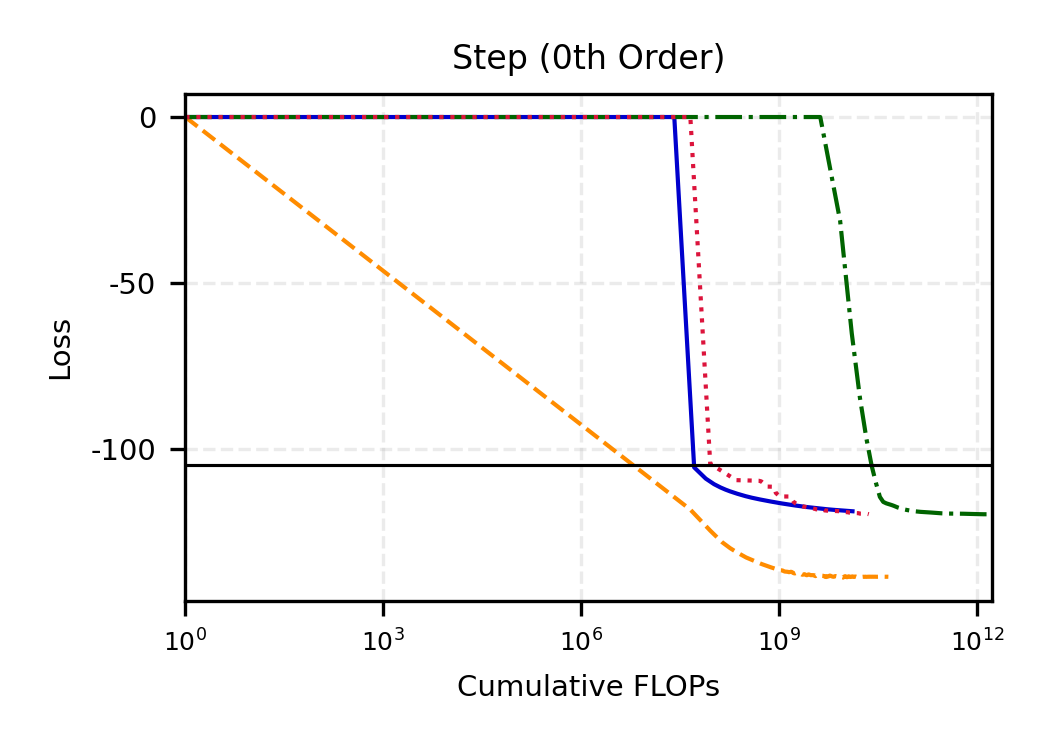
\includegraphics[width=.49\textwidth]{resources/optimization_algorithms/per_flop/StepFunction_order_0_loss_per_flop.png}
    \hfill
    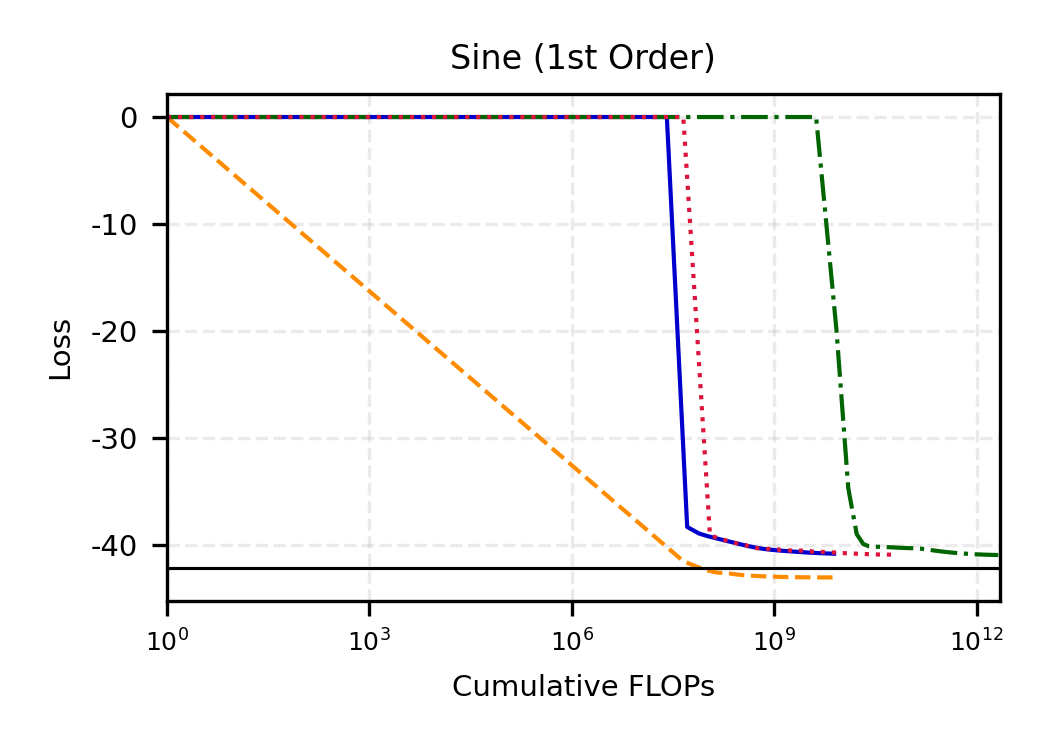
\includegraphics[width=.49\textwidth]{resources/optimization_algorithms/per_flop/Sinusoidal_order_1_loss_per_flop.png}
    
    \caption{Per-FLOP-normalized loss convergence across six DGPs. Panels (row-wise, left to right): (a) TN, (b) GS3, (c) GA3, (d) GS5, (e) Step, (f) Sine.}
    \label{fig:opt-per-flop-loss}
 \end{figure}
 
 \begin{figure}[H]
 \centering
 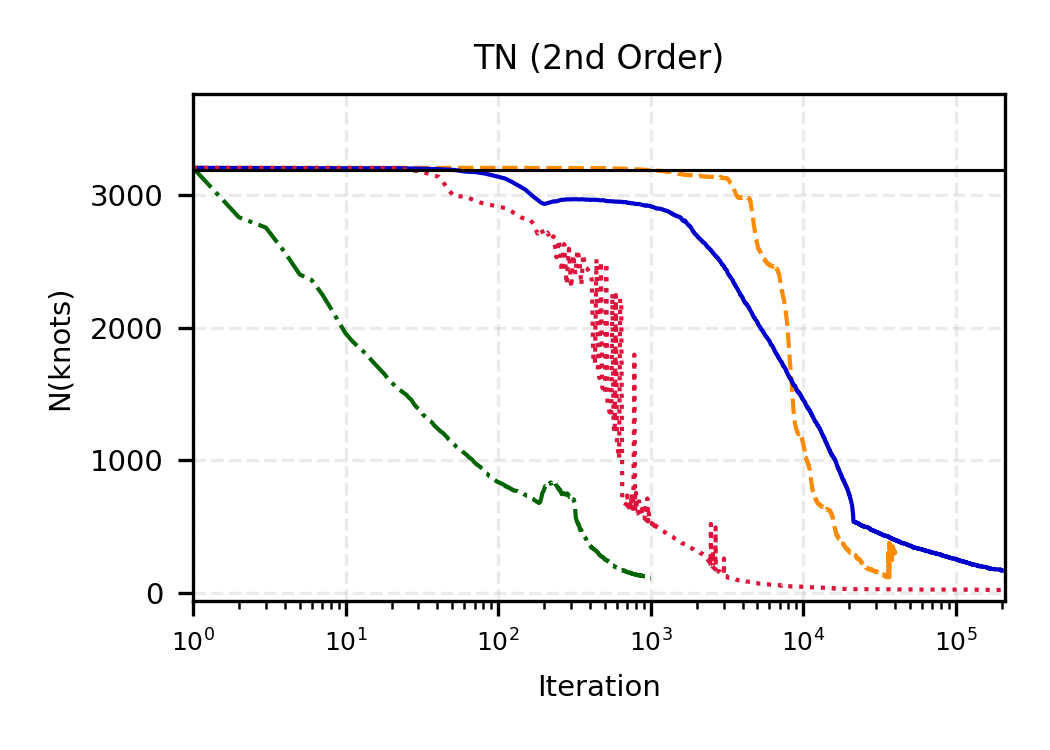
\includegraphics[width=.49\textwidth]{resources/optimization_algorithms/per_iter/TruncatedNormal_order_2_knot_selection.png}
 \hfill
 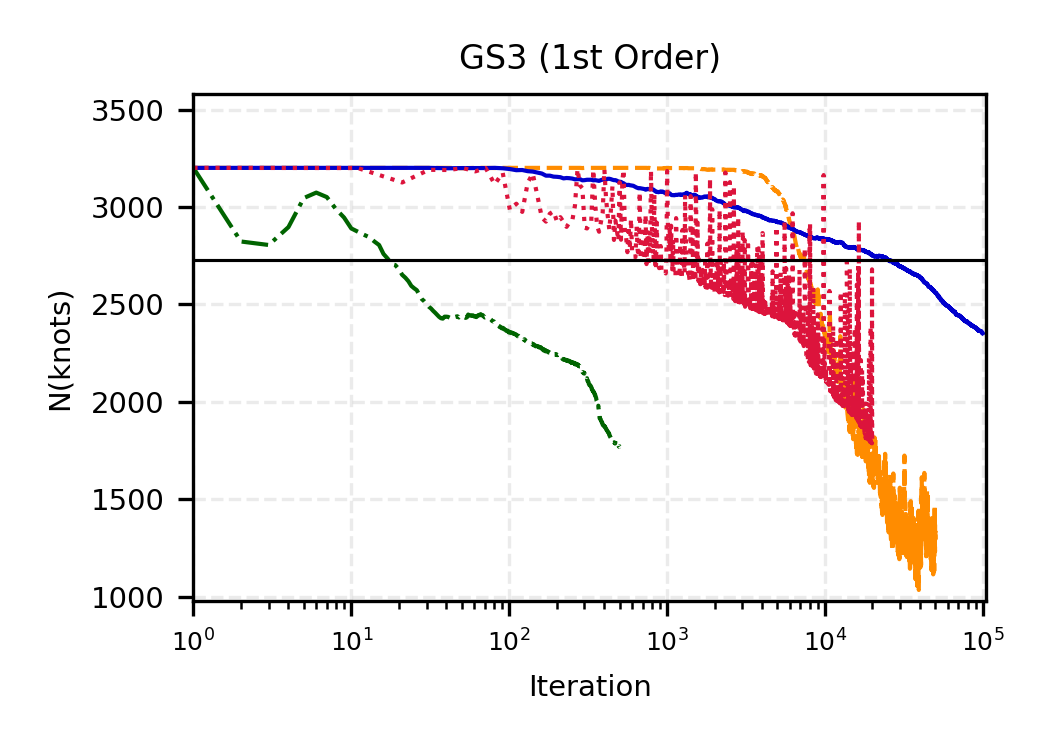
\includegraphics[width=.49\textwidth]{resources/optimization_algorithms/per_iter/TruncatedGMMSymmetricThree_order_1_knot_selection.png}
 
 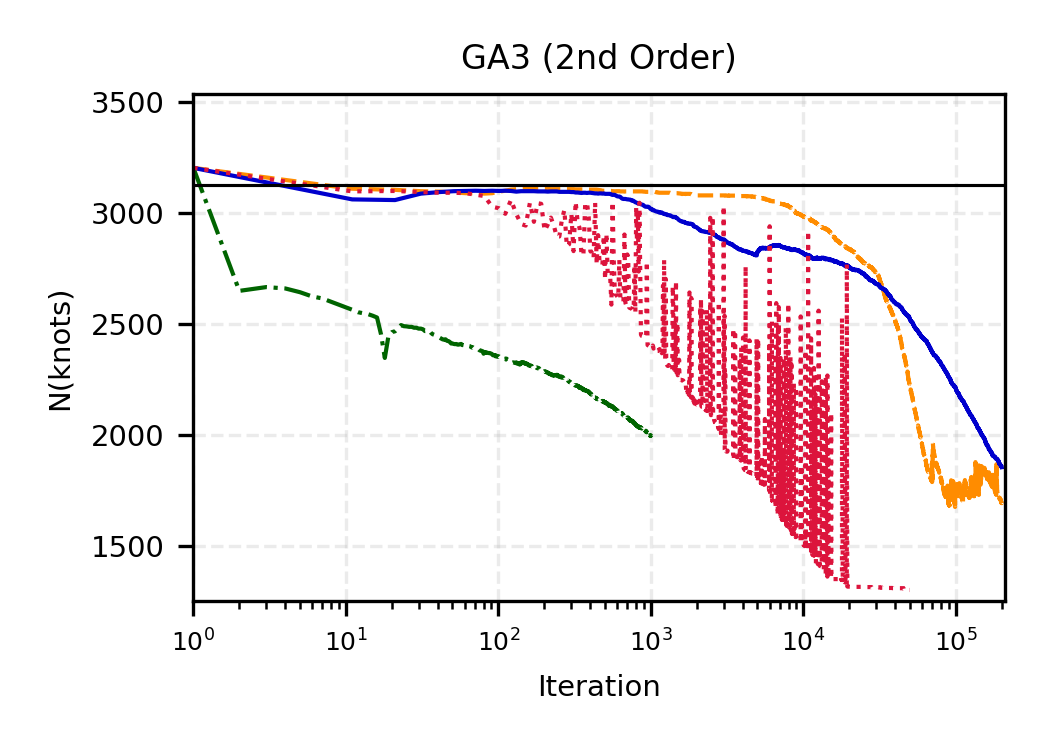
\includegraphics[width=.49\textwidth]{resources/optimization_algorithms/per_iter/TruncatedGMMAsymmetricThree_order_2_knot_selection.png}
 \hfill
 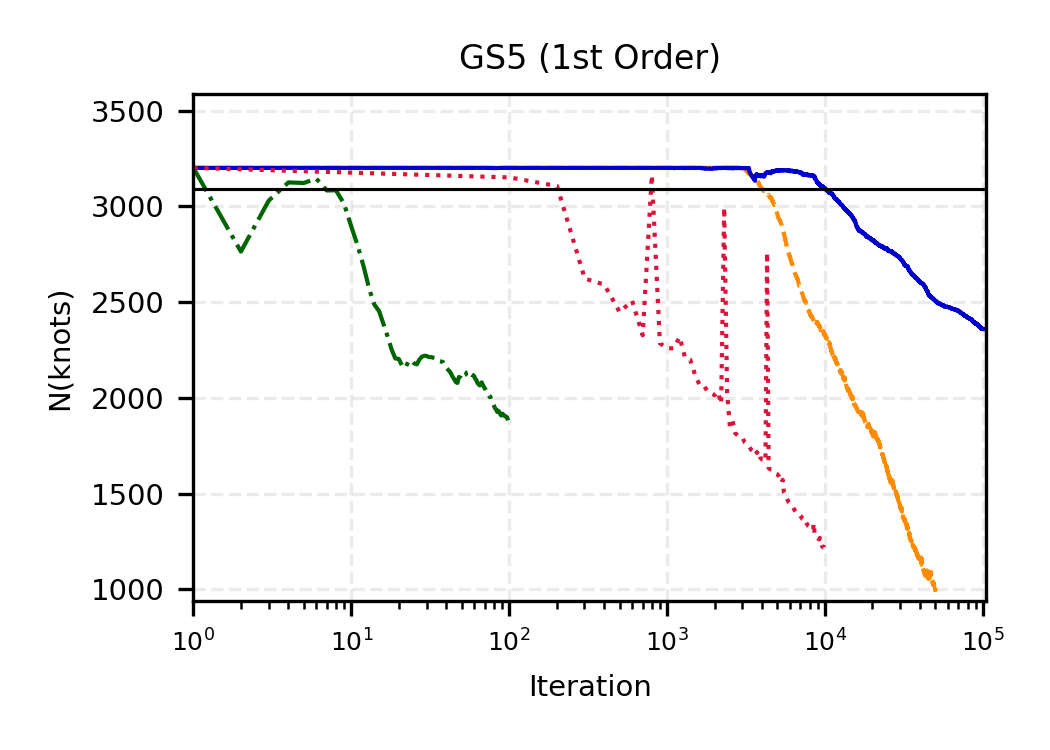
\includegraphics[width=.49\textwidth]{resources/optimization_algorithms/per_iter/TruncatedGMMFiveSpikes_order_1_knot_selection.png}
 
 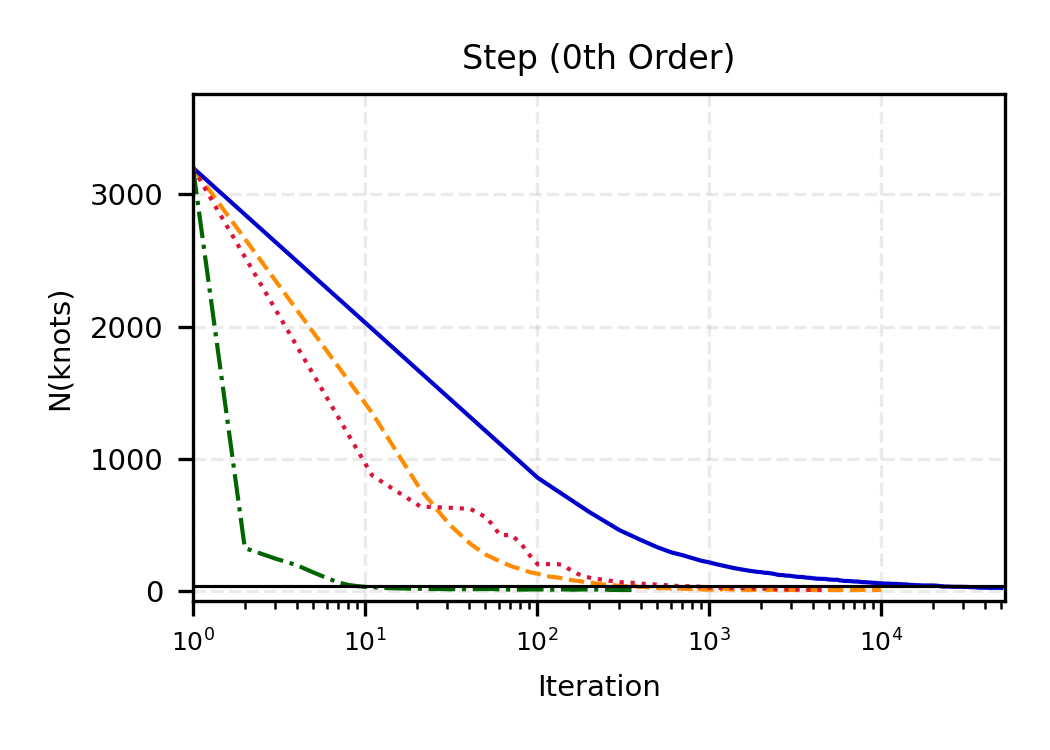
\includegraphics[width=.49\textwidth]{resources/optimization_algorithms/per_iter/StepFunction_order_0_knot_selection.png}
 \hfill
 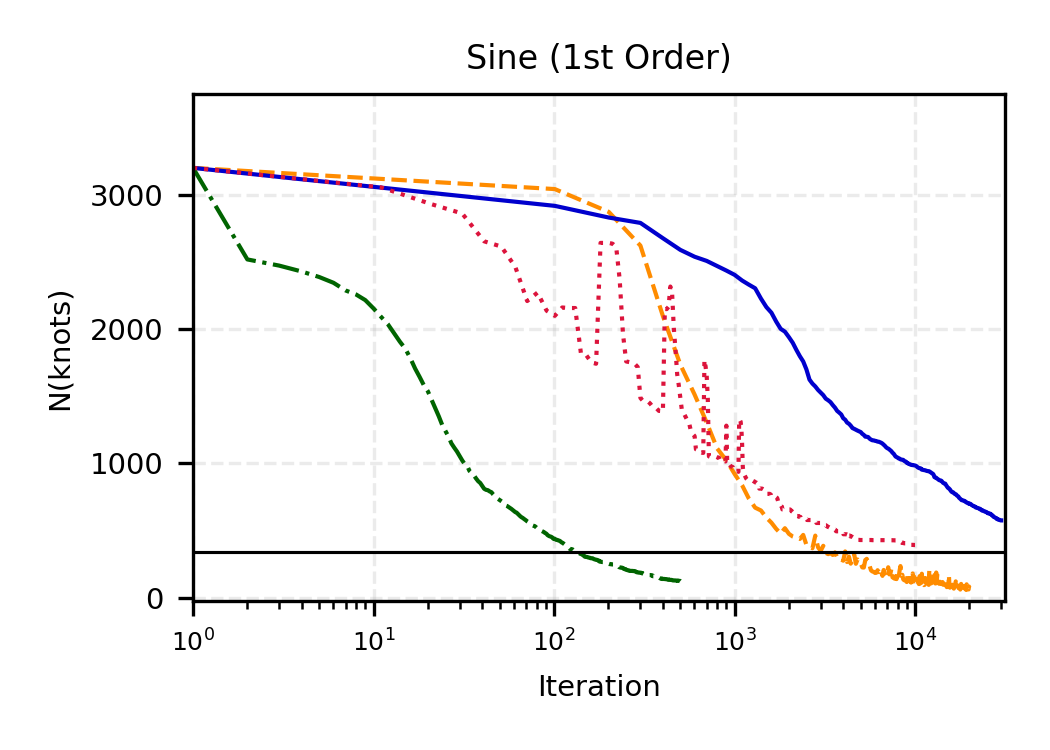
\includegraphics[width=.49\textwidth]{resources/optimization_algorithms/per_iter/Sinusoidal_order_1_knot_selection.png}
 
 \end{figure}
 
 \begin{figure}[H]
    \centering
    
\includegraphics[width=.9\textwidth]{resources/optimization_algorithms/per_iter/legend_knot_selection_algorithms.png}
    \caption{Per-iteration knot selection for optimization algorithms across six DGPs. Panels (row-wise, left to right): (a) TN, (b) GS3, (c) GA3, (d) GS5, (e) Step, (f) Sine.}
 \label{fig:opt-per-iter-knot}
 \end{figure}
 
 \begin{figure}[H]
 \centering
 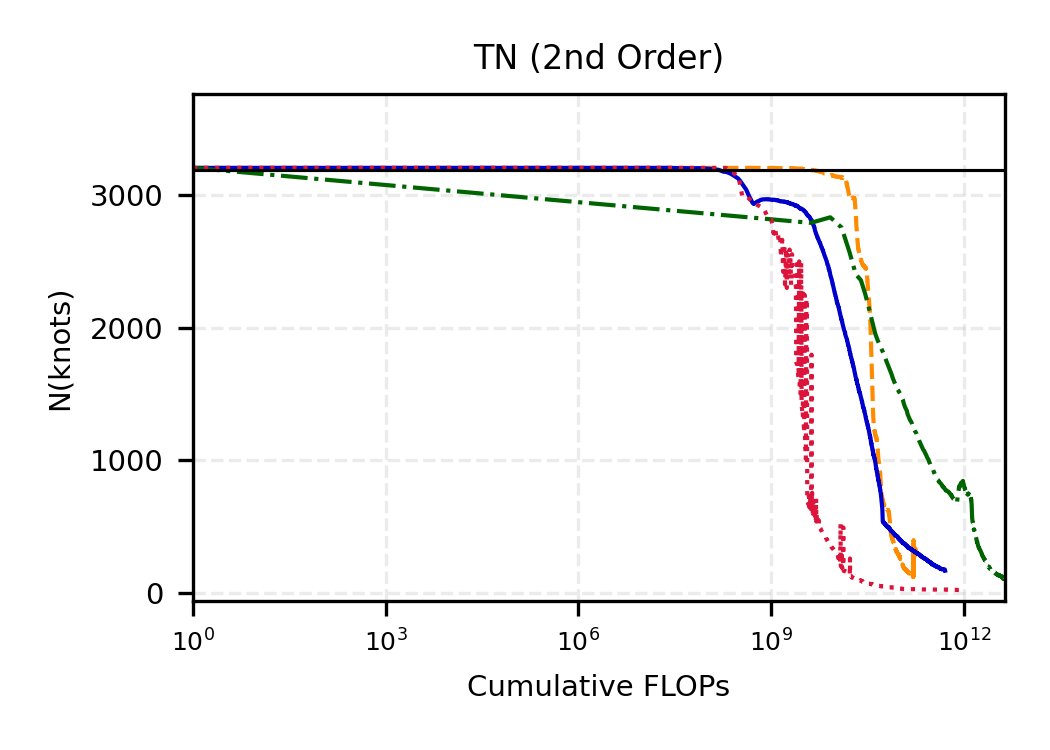
\includegraphics[width=.49\textwidth]{resources/optimization_algorithms/per_flop/TruncatedNormal_order_2_knot_selection_flops.png}
 \hfill
 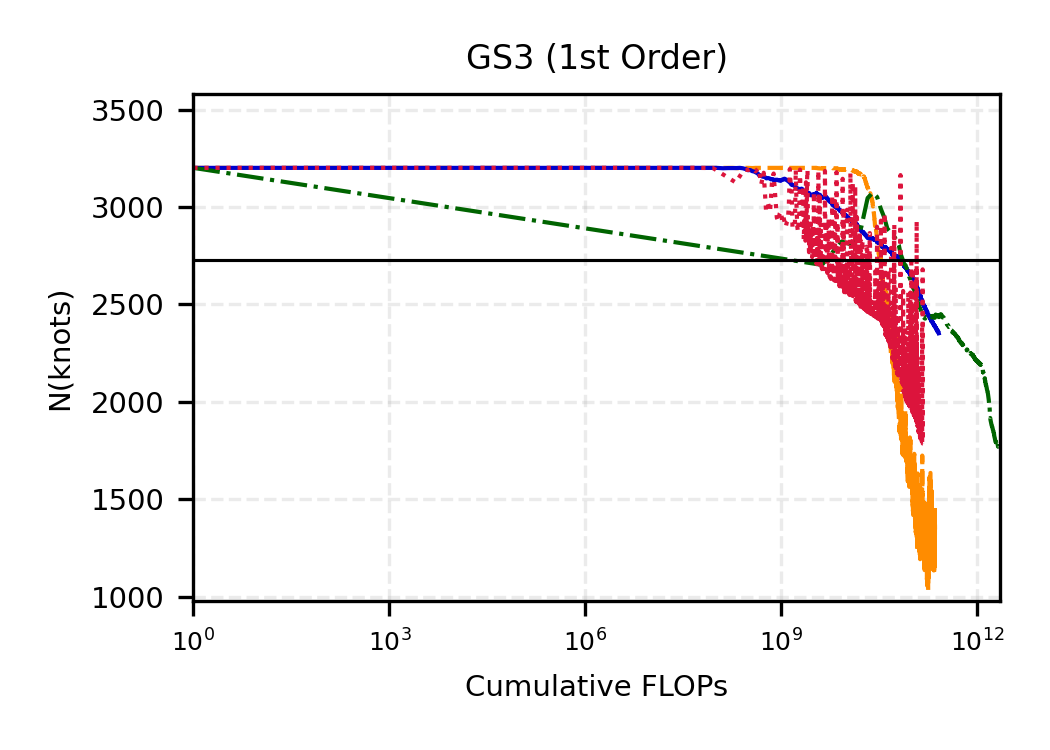
\includegraphics[width=.49\textwidth]{resources/optimization_algorithms/per_flop/TruncatedGMMSymmetricThree_order_1_knot_selection_flops.png}
 
 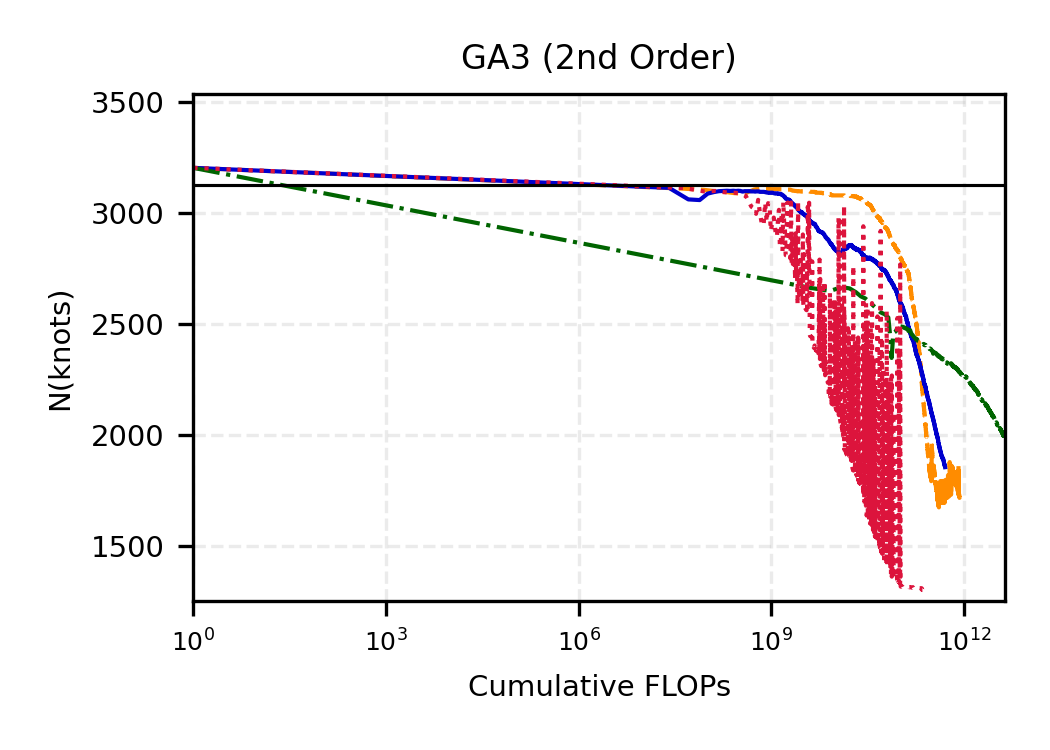
\includegraphics[width=.49\textwidth]{resources/optimization_algorithms/per_flop/TruncatedGMMAsymmetricThree_order_2_knot_selection_flops.png}
 \hfill
 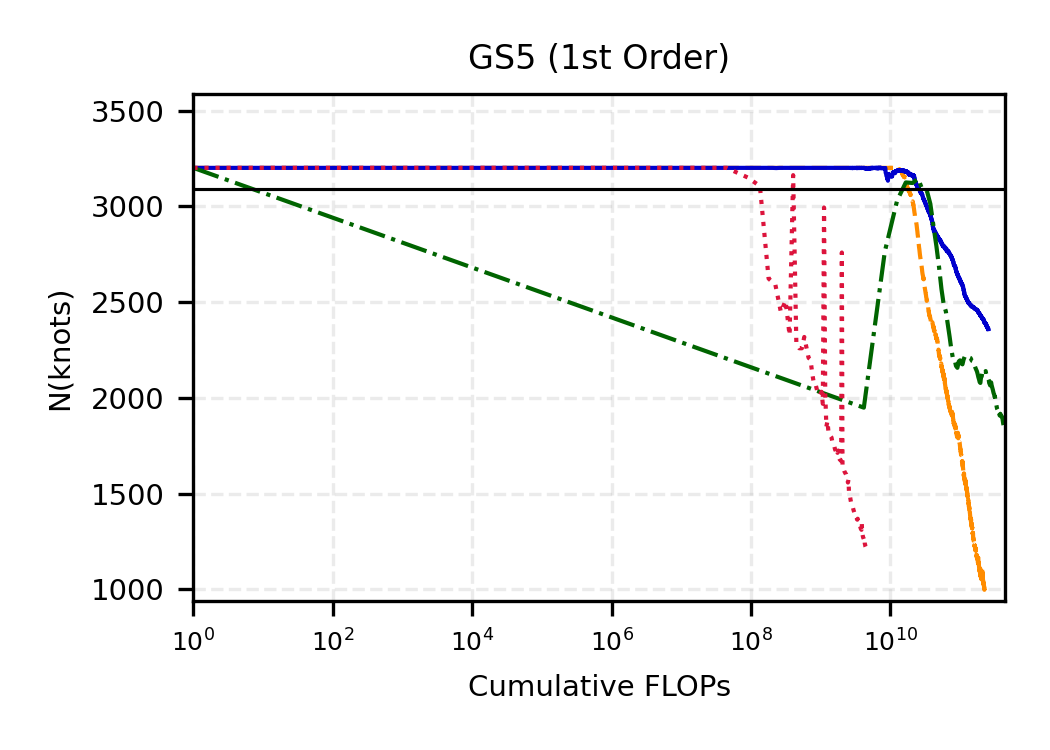
\includegraphics[width=.49\textwidth]{resources/optimization_algorithms/per_flop/TruncatedGMMFiveSpikes_order_1_knot_selection_flops.png}
 
 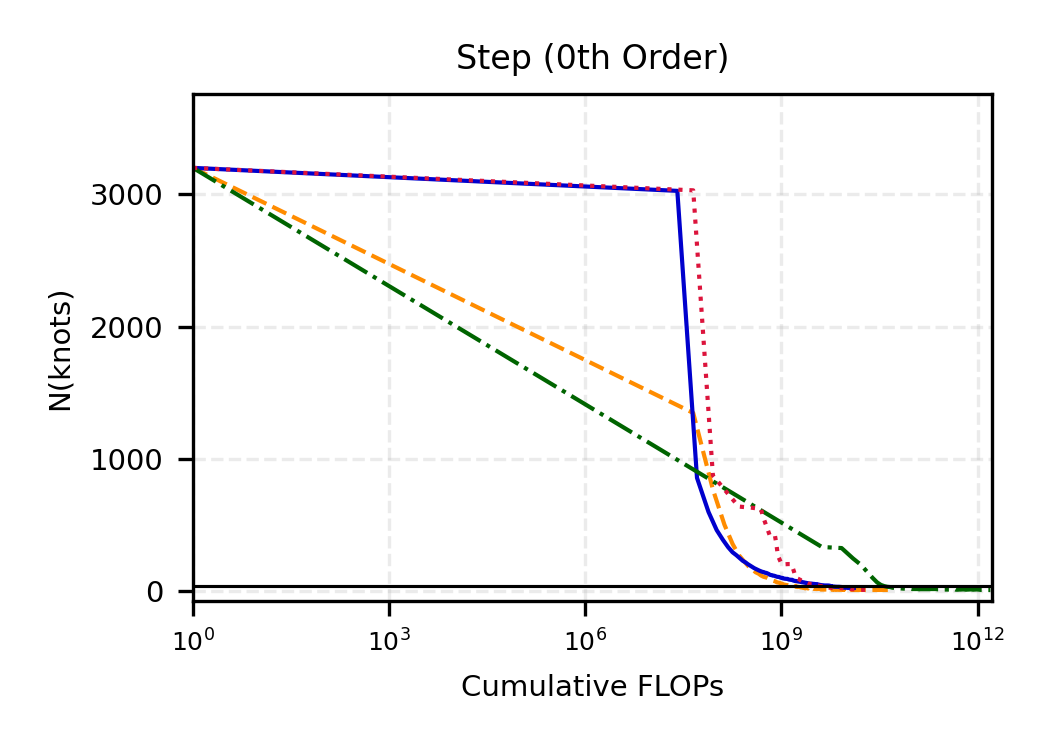
\includegraphics[width=.49\textwidth]{resources/optimization_algorithms/per_flop/StepFunction_order_0_knot_selection_flops.png}
 \hfill
 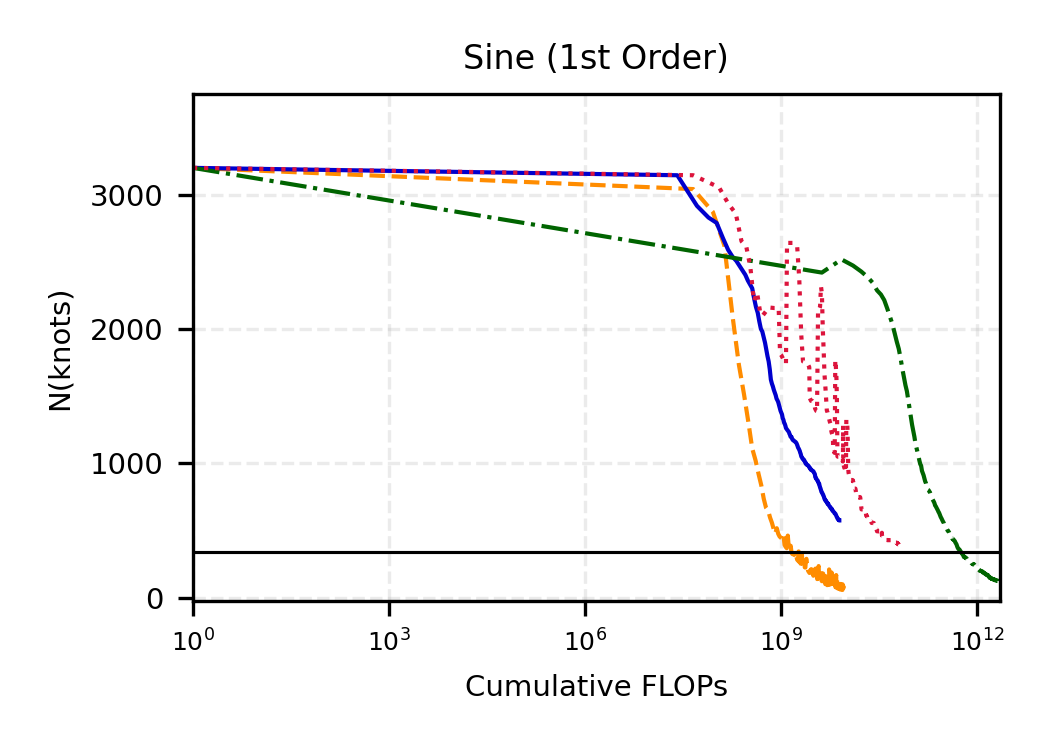
\includegraphics[width=.49\textwidth]{resources/optimization_algorithms/per_flop/Sinusoidal_order_1_knot_selection_flops.png}
 \end{figure}
 
 \begin{figure}[H]
    \centering
    
\includegraphics[width=.9\textwidth]{resources/optimization_algorithms/per_iter/legend_knot_selection_algorithms.png}
    \caption{Per-FLOP-normalized knot selection across six DGPs. Panels (row-wise, left to right): (a) TN, (b) GS3, (c) GA3, (d) GS5, (e) Step, (f) Sine.}
    \label{fig:opt-per-flop-knot}
 \end{figure}
 